\section*{Problema 19.08, S}

Dentro de la pared de una casa, una sección de tubería e agua caliente en forma de $L$ consiste en una pieza recta horizontal de $28cm$ de largo, un codo y una pieza recta vertical de $134cm$ de largo. Una trabe y un castillo mantienen fijos los extremos de esa sección de tubería de cobre. Encuentre la magnitudy dirección del desplazamiento del codo cuando hay flujo de agua, lo que eleva la temperatura de la tubería de $18^o C$ a $46.5^o C$.



\begin{figure}[H]
	\centering
	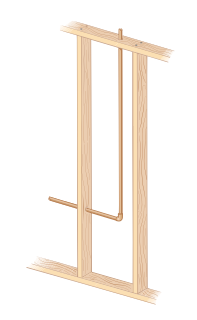
\includegraphics[scale=0.5]{./img/tubo.png}
	\caption{P19.08S}
\end{figure}



%%%%